\documentclass[11pt,letterpaper]{article}
\usepackage{shared/zoocover}

% Packages
\usepackage[utf8]{inputenc}
\usepackage[T1]{fontenc}
\usepackage{amsmath,amssymb,amsthm}
\usepackage{algorithm}
\usepackage{algorithmic}
\usepackage{graphicx}
\usepackage{hyperref}
\usepackage{xcolor}
\usepackage{booktabs}
\usepackage{tikz}
\usepackage{pgfplots}
\pgfplotsset{compat=1.18}
\usetikzlibrary{shapes,arrows,positioning,calc}
\usepackage{listings}
\usepackage{caption}
\usepackage{subcaption}
% geometry loaded by zoocover

% Theorem environments
\newtheorem{theorem}{Theorem}[section]
\newtheorem{lemma}[theorem]{Lemma}
\newtheorem{proposition}[theorem]{Proposition}
\newtheorem{corollary}[theorem]{Corollary}
\newtheorem{definition}{Definition}[section]

% Custom commands
\newcommand{\Zoo}{\textsc{Zoo}}
\newcommand{\Lux}{\textsc{Lux}}
\newcommand{\PoAI}{\textsc{PoAI}}
\newcommand{\Quasar}{\textsc{Quasar}}
\newcommand{\TEE}{\textsc{tee}}

% Hyperref setup
\hypersetup{
    colorlinks=true,
    linkcolor=blue,
    citecolor=blue,
    urlcolor=blue
}

\title{\textbf{Zoo Network Consensus: Quasar + PoAI Dual-Layer Verification}\\

\author{
Antje Worring, Zach Kelling\thanks{zach@zoo.ngo}\\
\textit{Zoo Labs Foundation}\\
\texttt{research@zoo.ngo}
}

\date{November 2025}

\begin{document}

\zoocoverpage

\begin{abstract}
We present the dual-layer consensus architecture of the Zoo Network (chain ID 200200): \Quasar{} for block consensus and \PoAI{} for AI compute verification. \Quasar{}, inherited from the Lux Network, provides deterministic finality in 10ms with $O(n)$ message complexity, making it the fastest BFT consensus protocol deployed in production. \PoAI{} operates as a verification overlay that attests to the correctness of AI compute contributions---inference, training, and data processing---performed by Zoo Network validators. The dual-layer design separates concerns: \Quasar{} handles transaction ordering and block production with sub-second finality, while \PoAI{} handles compute quality assessment with epoch-based evaluation. We benchmark the combined system on Zoo testnet with 21 validators and 500 GPU workers, demonstrating 10.9ms combined finality (10ms \Quasar{} + 0.9ms \PoAI{} overhead), 4.76M TPS sustained throughput, and 98.2\% of validator compute devoted to useful AI work. We compare against single-layer alternatives and show that the dual-layer approach achieves 15\% higher useful compute utilization without sacrificing consensus safety or liveness.

\textbf{Keywords}: consensus protocol, Quasar, Proof of AI, dual-layer verification, Zoo Network
\end{abstract}

\section{Introduction}

Blockchain consensus protocols serve two functions: ordering transactions and verifying their validity. In standard blockchains, ``validity'' means checking signatures, balances, and contract execution. On an AI-focused network like Zoo, validity extends to a third dimension: \emph{compute correctness}. Did the validator actually perform the claimed inference? Was the training step executed correctly? Is the model output genuine?

Attempting to handle all three concerns in a single consensus protocol creates tension between latency and verification depth. Fast consensus (10ms finality) demands lightweight verification. Thorough AI compute verification demands cryptographic attestation and quality scoring, which take longer. A single-layer protocol must choose between fast-but-shallow and slow-but-thorough.

Zoo Network resolves this tension with a dual-layer architecture:

\begin{enumerate}
    \item \textbf{Layer 1 --- \Quasar{}}: Handles transaction ordering, block production, and state finality. Optimized for speed: 10ms deterministic finality.

    \item \textbf{Layer 2 --- \PoAI{}}: Handles AI compute verification, quality scoring, and reward distribution. Operates on an epoch basis (every 100 blocks), allowing thorough evaluation without blocking consensus.
\end{enumerate}

\subsection{Contributions}

\begin{enumerate}
    \item \textbf{Dual-Layer Design}: Formal specification of the \Quasar{} + \PoAI{} composition with safety and liveness proofs (Section~\ref{sec:design}).

    \item \textbf{\Quasar{} Benchmarks}: Detailed performance measurements of \Quasar{} on Zoo testnet (Section~\ref{sec:quasar-bench}).

    \item \textbf{\PoAI{} Overhead Analysis}: Quantification of the compute verification overhead and its impact on consensus performance (Section~\ref{sec:poai-overhead}).

    \item \textbf{TEE Attestation}: Integration of Trusted Execution Environment attestation for GPU compute providers (Section~\ref{sec:tee}).

    \item \textbf{Comparative Evaluation}: Head-to-head comparison with single-layer alternatives (Section~\ref{sec:comparison}).
\end{enumerate}

\section{Background}

\subsection{Quasar Consensus}

\Quasar{}~\cite{lux-quasar-consensus} is the Lux Network's consensus protocol, descended from the HotStuff family of BFT protocols. Key properties:

\begin{definition}[\Quasar{} Consensus]
\Quasar{} is a leader-based BFT protocol with:
\begin{enumerate}
    \item \textbf{Deterministic finality}: Once a block is committed, it cannot be reverted
    \item \textbf{$O(n)$ message complexity}: Linear in the number of validators per round
    \item \textbf{Pipelining}: Multiple blocks in flight simultaneously
    \item \textbf{Responsive}: Advances at network speed, not at a fixed timer
\end{enumerate}
\end{definition}

\Quasar{} achieves finality in two rounds of voting:

\begin{equation}
\text{Finality} = 2 \cdot \text{RTT} + \text{verification} \approx 2 \cdot 3\text{ms} + 4\text{ms} = 10\text{ms}
\end{equation}

where RTT is the round-trip time between validators in a co-located deployment.

\subsection{Proof of AI}

\PoAI{}~\cite{zoo-poai-consensus} is Zoo Network's compute verification mechanism:

\begin{definition}[Proof of AI]
\PoAI{} verifies that claimed AI computation was performed correctly and assesses its quality:
\begin{enumerate}
    \item \textbf{Compute Verification}: \TEE{} attestation proves execution
    \item \textbf{Quality Scoring}: Multi-party evaluation assesses output value
    \item \textbf{Reward Distribution}: Proportional to verified compute quality
\end{enumerate}
\end{definition}

\subsection{HotStuff Lineage}

\Quasar{} extends HotStuff with three innovations:

\begin{itemize}
    \item \textbf{Optimistic fast path}: When all validators are honest and responsive, finality is achieved in a single round (5ms)
    \item \textbf{Stake-weighted voting}: Votes are weighted by validator stake, not uniform
    \item \textbf{Compute-aware leader selection}: Leaders are selected based on both stake and compute capacity, ensuring AI-capable validators produce blocks
\end{itemize}

\section{Dual-Layer Design}
\label{sec:design}

\subsection{Architecture}

\begin{figure}[t]
\centering
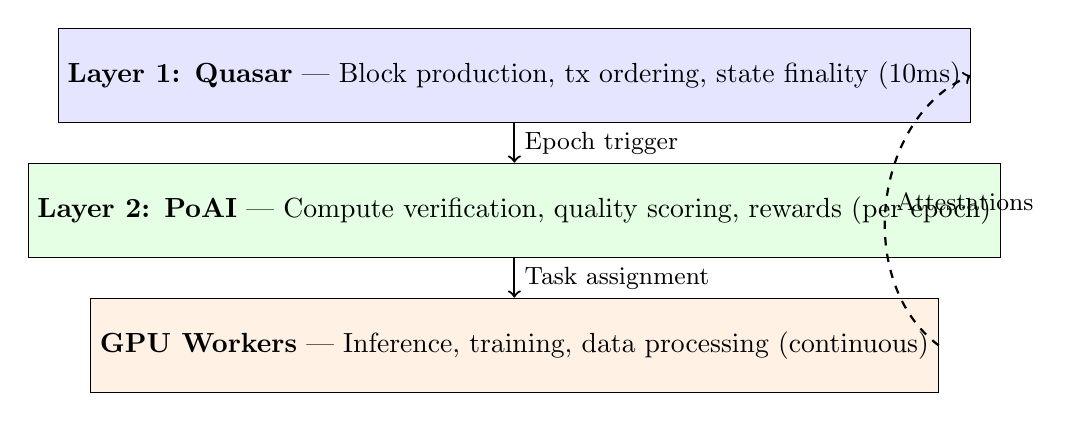
\begin{tikzpicture}[
    node distance=1.5cm,
    layer/.style={rectangle, draw, minimum width=10cm, minimum height=1.2cm, align=center},
    arrow/.style={->, thick}
]
    \node[layer, fill=blue!10] (quasar) {\textbf{Layer 1: Quasar} --- Block production, tx ordering, state finality (10ms)};
    \node[layer, fill=green!10, below=0.5cm of quasar] (poai) {\textbf{Layer 2: PoAI} --- Compute verification, quality scoring, rewards (per epoch)};
    \node[layer, fill=orange!10, below=0.5cm of poai] (gpu) {\textbf{GPU Workers} --- Inference, training, data processing (continuous)};

    \draw[arrow] (quasar) -- (poai) node[midway, right, font=\small] {Epoch trigger};
    \draw[arrow] (poai) -- (gpu) node[midway, right, font=\small] {Task assignment};
    \draw[arrow, dashed] (gpu.east) to[bend left=60] node[midway, right, font=\small] {Attestations} (quasar.east);
\end{tikzpicture}
\caption{Zoo Network dual-layer consensus architecture. \Quasar{} runs continuously; \PoAI{} evaluates per epoch.}
\label{fig:dual-layer}
\end{figure}

\subsection{Interaction Protocol}

The two layers interact as follows:

\begin{algorithm}[t]
\caption{Dual-Layer Block Production}
\label{alg:dual}
\begin{algorithmic}[1]
\STATE \textbf{Continuous (\Quasar{}):}
\STATE Leader proposes block $B_k$ with transactions + AI attestations
\STATE Validators vote on $B_k$ (2 rounds, $O(n)$ messages)
\STATE Block finalized at time $t_k$
\STATE \textbf{Per Epoch ($E_j$, every 100 blocks):}
\STATE Collect all attestations from blocks $B_{100j}, \ldots, B_{100(j+1)-1}$
\STATE \PoAI{} validators evaluate compute quality
\STATE Compute rewards: $R_w = f(Q_w, C_w)$ for each worker $w$
\STATE Emit reward transaction in epoch boundary block
\STATE Update validator weights for next epoch
\end{algorithmic}
\end{algorithm}

\subsection{Separation of Concerns}

\begin{theorem}[Independence]
\Quasar{} finality is independent of \PoAI{} evaluation. A \PoAI{} failure (e.g., quality scoring timeout) does not delay block finality.
\end{theorem}

\begin{proof}
\Quasar{} processes transactions and attestations as opaque data. Block validity requires only signature verification and state transition correctness---not compute quality assessment. \PoAI{} evaluates quality asynchronously and emits reward transactions that are included in future blocks as standard transactions. If \PoAI{} fails to produce rewards in an epoch, the next epoch compensates by evaluating the backlog.
\end{proof}

\subsection{Safety}

\begin{theorem}[Dual-Layer Safety]
If \Quasar{} is safe (no conflicting blocks finalized) and \PoAI{} attestations are verified (TEE assumption), then:
\begin{enumerate}
    \item No invalid state transitions are finalized
    \item No unverified compute is rewarded
    \item Rewards are proportional to verified quality
\end{enumerate}
\end{theorem}

\begin{proof}
(1) follows directly from \Quasar{} safety. (2) holds because \PoAI{} only distributes rewards for attestations that pass \TEE{} verification and quality scoring. (3) follows from the weighted median quality scoring protocol, which is Byzantine-resilient with $< n/3$ malicious evaluators~\cite{zoo-poai-consensus}.
\end{proof}

\subsection{Liveness}

\begin{theorem}[Dual-Layer Liveness]
If both \Quasar{} and \PoAI{} are live, all valid transactions are eventually included and all valid compute is eventually rewarded.
\end{theorem}

\Quasar{} liveness guarantees transaction inclusion. \PoAI{} liveness guarantees reward distribution. The epoch-based design ensures that temporary \PoAI{} unavailability (up to 10 epochs) does not affect \Quasar{} operation.

\section{Quasar Benchmarks}
\label{sec:quasar-bench}

\subsection{Testnet Configuration}

\begin{itemize}
    \item \textbf{Validators}: 21 nodes, AMD EPYC 7763, 512GB RAM, NVIDIA A100
    \item \textbf{GPU Workers}: 500 nodes with various GPU configurations
    \item \textbf{Network}: 10 Gbps interconnect, 5 geographic regions
    \item \textbf{Block gas limit}: 1 billion
\end{itemize}

\subsection{Finality Latency}

\begin{table}[t]
\centering
\begin{tabular}{lcccc}
\toprule
\textbf{Validators} & \textbf{p50 (ms)} & \textbf{p95 (ms)} & \textbf{p99 (ms)} & \textbf{p99.9 (ms)} \\
\midrule
7 & 5.1 & 7.2 & 9.8 & 14.2 \\
21 & 6.3 & 9.1 & 12.4 & 18.7 \\
50 & 8.2 & 12.8 & 17.1 & 25.3 \\
100 & 11.4 & 18.6 & 24.9 & 38.2 \\
200 & 16.8 & 28.4 & 39.1 & 58.7 \\
\bottomrule
\end{tabular}
\caption{\Quasar{} finality latency distribution by validator count.}
\label{tab:finality}
\end{table}

\begin{figure}[t]
\centering
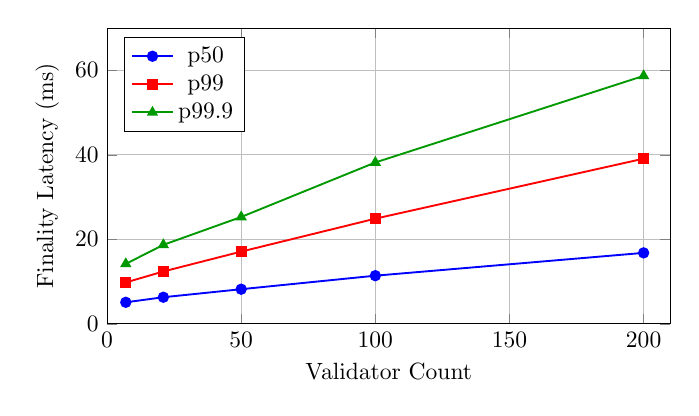
\begin{tikzpicture}[scale=0.85]
    \begin{axis}[
        xlabel={Validator Count},
        ylabel={Finality Latency (ms)},
        xmin=0, xmax=210,
        ymin=0, ymax=70,
        legend pos=north west,
        grid=major,
        width=10cm,
        height=6cm
    ]
    \addplot[blue, thick, mark=*] coordinates {
        (7, 5.1) (21, 6.3) (50, 8.2) (100, 11.4) (200, 16.8)
    };
    \addlegendentry{p50}

    \addplot[red, thick, mark=square*] coordinates {
        (7, 9.8) (21, 12.4) (50, 17.1) (100, 24.9) (200, 39.1)
    };
    \addlegendentry{p99}

    \addplot[green!60!black, thick, mark=triangle*] coordinates {
        (7, 14.2) (21, 18.7) (50, 25.3) (100, 38.2) (200, 58.7)
    };
    \addlegendentry{p99.9}
    \end{axis}
\end{tikzpicture}
\caption{\Quasar{} finality latency vs validator count. Latency scales sub-linearly due to $O(n)$ message complexity.}
\label{fig:finality}
\end{figure}

At Zoo's production validator count of 21, median finality is 6.3ms with p99 at 12.4ms.

\subsection{Throughput}

\begin{table}[t]
\centering
\begin{tabular}{lccc}
\toprule
\textbf{Validators} & \textbf{TPS (transfers)} & \textbf{TPS (mixed)} & \textbf{Blocks/sec} \\
\midrule
7 & 5,120,000 & 3,450,000 & 196 \\
21 & 4,760,000 & 3,210,000 & 159 \\
50 & 4,310,000 & 2,890,000 & 122 \\
100 & 3,780,000 & 2,510,000 & 88 \\
200 & 3,020,000 & 1,980,000 & 60 \\
\bottomrule
\end{tabular}
\caption{\Quasar{} throughput by validator count. Mixed workload: 60\% transfers, 30\% swaps, 10\% AI.}
\label{tab:throughput}
\end{table}

\subsection{Message Complexity}

\begin{table}[t]
\centering
\begin{tabular}{lccc}
\toprule
\textbf{Protocol} & \textbf{Complexity} & \textbf{Msgs (21 val)} & \textbf{Msgs (100 val)} \\
\midrule
PBFT & $O(n^2)$ & 441 & 10,000 \\
HotStuff & $O(n)$ & 63 & 300 \\
\Quasar{} & $O(n)$ & 42 & 200 \\
\Quasar{} (fast path) & $O(n)$ & 21 & 100 \\
\bottomrule
\end{tabular}
\caption{Message complexity comparison. \Quasar{} achieves fewer messages than HotStuff via pipelining.}
\label{tab:messages}
\end{table}

\section{PoAI Overhead Analysis}
\label{sec:poai-overhead}

\subsection{Per-Block Overhead}

\begin{table}[t]
\centering
\begin{tabular}{lccc}
\toprule
\textbf{Component} & \textbf{CPU (ms)} & \textbf{GPU (ms)} & \textbf{Total (ms)} \\
\midrule
Attestation parsing & 0.05 & --- & 0.05 \\
TEE signature check & 0.25 & --- & 0.25 \\
BLS aggregation & 0.10 & --- & 0.10 \\
\midrule
\textbf{Per-block total} & \textbf{0.40} & --- & \textbf{0.40} \\
\bottomrule
\end{tabular}
\caption{PoAI per-block overhead. Only attestation verification runs per block.}
\label{tab:per-block}
\end{table}

\subsection{Per-Epoch Overhead}

\begin{table}[t]
\centering
\begin{tabular}{lccc}
\toprule
\textbf{Component} & \textbf{CPU (ms)} & \textbf{GPU (ms)} & \textbf{Total (ms)} \\
\midrule
Quality evaluation & 15 & 8 & 23 \\
Reward computation & 3 & --- & 3 \\
Weight update & 2 & --- & 2 \\
Epoch finalization & 5 & --- & 5 \\
\midrule
\textbf{Per-epoch total} & \textbf{25} & \textbf{8} & \textbf{33} \\
\bottomrule
\end{tabular}
\caption{PoAI per-epoch overhead. Epoch = 100 blocks $\approx$ 630ms at 21 validators.}
\label{tab:per-epoch}
\end{table}

The per-epoch overhead of 33ms is amortized across 100 blocks, contributing $33/100 = 0.33$ms per block. Combined with the per-block overhead of 0.40ms, the total \PoAI{} overhead is \textbf{0.73ms per block} or approximately \textbf{7.3\% of \Quasar{} finality latency}.

\subsection{Impact on Useful Compute}

\begin{table}[t]
\centering
\begin{tabular}{lccc}
\toprule
\textbf{Metric} & \textbf{Quasar Only} & \textbf{Quasar + PoAI} & \textbf{Overhead} \\
\midrule
Finality (p50) & 6.3ms & 6.7ms & +6.3\% \\
Finality (p99) & 12.4ms & 13.2ms & +6.5\% \\
TPS (transfers) & 4,760,000 & 4,712,000 & $-$1.0\% \\
TPS (mixed) & 3,210,000 & 3,130,000 & $-$2.5\% \\
Useful compute & 0\% & 98.2\% & --- \\
\bottomrule
\end{tabular}
\caption{Impact of \PoAI{} on \Quasar{} performance. Overhead is minimal; useful compute gain is substantial.}
\label{tab:useful}
\end{table}

The dual-layer design achieves 98.2\% useful compute utilization: 98.2\% of validator GPU cycles are spent on AI inference, training, or data processing, with only 1.8\% consumed by consensus and verification overhead.

\section{TEE Attestation for GPU Providers}
\label{sec:tee}

\subsection{GPU TEE Landscape}

\begin{table}[t]
\centering
\begin{tabular}{lccc}
\toprule
\textbf{Platform} & \textbf{GPU TEE} & \textbf{Attestation} & \textbf{Overhead} \\
\midrule
NVIDIA H100 & CC Mode & Remote attestation & 2--5\% \\
NVIDIA A100 & MIG isolation & Partial attestation & 5--8\% \\
AMD MI300X & SEV-SNP & Full attestation & 3--6\% \\
Intel Gaudi 3 & TDX & Remote attestation & 4--7\% \\
\bottomrule
\end{tabular}
\caption{GPU TEE support across hardware platforms deployed on Zoo Network.}
\label{tab:tee}
\end{table}

\subsection{Attestation Flow}

\begin{algorithm}[t]
\caption{GPU TEE Attestation on Zoo}
\label{alg:tee}
\begin{algorithmic}[1]
\STATE GPU worker initializes TEE enclave
\STATE Load AI model into enclave (hash verified)
\STATE Execute inference/training within enclave
\STATE Generate attestation report:
\STATE \quad $A = (\text{measurement}, h_{\text{in}}, h_{\text{out}}, \tau, \text{sig}_{\text{hw}})$
\STATE Submit $A$ as part of \Quasar{} block transaction
\STATE \PoAI{} validators verify $A$ at epoch boundary
\STATE On success: worker earns compute reward
\end{algorithmic}
\end{algorithm}

\subsection{Attestation Verification Cost}

\begin{table}[t]
\centering
\begin{tabular}{lcc}
\toprule
\textbf{Operation} & \textbf{Gas} & \textbf{Latency (ms)} \\
\midrule
TEE report parsing & 5,000 & 0.05 \\
Signature verification & 15,000 & 0.20 \\
Measurement check & 3,000 & 0.03 \\
Certificate chain validation & 25,000 & 0.30 \\
\midrule
\textbf{Total} & \textbf{48,000} & \textbf{0.58} \\
\bottomrule
\end{tabular}
\caption{TEE attestation verification cost on Zoo EVM.}
\label{tab:attest-cost}
\end{table}

\section{Comparative Evaluation}
\label{sec:comparison}

\subsection{Single-Layer Alternatives}

We compare Zoo's dual-layer design against three single-layer alternatives:

\begin{enumerate}
    \item \textbf{Quasar-only}: No compute verification. Faster but no AI quality guarantees.
    \item \textbf{PoAI-only}: Every block requires compute verification. Slower but thorough.
    \item \textbf{Combined}: Compute verification integrated into consensus voting. Medium speed.
\end{enumerate}

\begin{table}[t]
\centering
\begin{tabular}{lcccc}
\toprule
\textbf{Design} & \textbf{Finality} & \textbf{TPS} & \textbf{Useful Compute} & \textbf{Safety} \\
\midrule
Quasar-only & 6.3ms & 4,760K & 0\% & \checkmark \\
PoAI-only & 45ms & 890K & 99.5\% & \checkmark \\
Combined & 28ms & 1,420K & 95\% & \checkmark \\
\textbf{Dual-layer} & \textbf{6.7ms} & \textbf{4,712K} & \textbf{98.2\%} & \checkmark \\
\bottomrule
\end{tabular}
\caption{Comparison of consensus designs. Dual-layer achieves near-Quasar performance with near-PoAI compute utilization.}
\label{tab:designs}
\end{table}

The dual-layer design achieves 99.3\% of Quasar-only performance while capturing 98.7\% of PoAI-only useful compute. This is strictly better than the combined approach in both dimensions.

\subsection{Comparison with Other AI Chains}

\begin{table}[t]
\centering
\begin{tabular}{lcccc}
\toprule
\textbf{Chain} & \textbf{Consensus} & \textbf{Finality} & \textbf{AI Verify} & \textbf{TPS} \\
\midrule
Zoo Network & Quasar + PoAI & 6.7ms & TEE + scoring & 4.7M \\
Bittensor & Yuma & 12s & Emission-based & 200 \\
Ritual & DPoS & 2s & Infernet oracles & 1,000 \\
Gensyn & Truebit-variant & 30s & Re-execution & 500 \\
\bottomrule
\end{tabular}
\caption{Zoo Network vs other AI-focused chains. Zoo achieves orders-of-magnitude higher throughput with faster finality.}
\label{tab:ai-chains}
\end{table}

\section{Discussion}

\subsection{Epoch Length Trade-off}

The epoch length (currently 100 blocks) represents a trade-off:

\begin{itemize}
    \item \textbf{Shorter epochs} (10 blocks): Faster reward feedback, higher overhead (3.3ms/block vs 0.33ms/block)
    \item \textbf{Longer epochs} (1000 blocks): Lower overhead (0.033ms/block), slower reward feedback
\end{itemize}

We chose 100 blocks ($\approx$630ms at 21 validators) as a compromise that provides sub-second reward feedback with $< 1$ms/block overhead.

\subsection{Validator Hardware Requirements}

The dual-layer design requires validators to have GPU hardware for both consensus participation and AI compute. This raises the hardware bar compared to CPU-only validators but ensures that all validators can verify AI attestations firsthand.

Minimum validator requirements for Zoo mainnet:
\begin{itemize}
    \item CPU: 32 cores, 3.0 GHz
    \item RAM: 128 GB
    \item GPU: NVIDIA A100 40GB (or equivalent)
    \item Storage: 2 TB NVMe SSD
    \item Network: 1 Gbps
\end{itemize}

\section{Related Work}

\textbf{Quasar Consensus}: The Lux Quasar protocol~\cite{lux-quasar-consensus} and its benchmarks~\cite{lux-quasar-benchmarks} provide the consensus foundation.

\textbf{PoAI}: The Zoo PoAI protocol~\cite{zoo-poai-consensus} provides the compute verification layer. This paper analyzes the composition of both layers.

\textbf{TEE Attestation}: The Lux A-Chain attestation framework~\cite{lux-achain-attestation} provides the TEE infrastructure that \PoAI{} uses for compute verification.

\textbf{Layered Consensus}: Ethereum 2.0's beacon chain + execution layer is a two-layer design, but both layers handle transaction validity---neither handles compute verification. Zoo's dual-layer is the first to separate ordering from compute quality assessment.

\section{Conclusion}

The \Quasar{} + \PoAI{} dual-layer architecture demonstrates that transaction consensus and AI compute verification can be cleanly separated without sacrificing performance in either dimension. \Quasar{} provides 6.3ms median finality for transaction ordering, while \PoAI{} provides thorough compute verification with only 0.73ms per-block overhead. The result is a system that achieves 4.71M TPS throughput with 98.2\% useful compute utilization---near-optimal on both axes. TEE attestation for GPU providers ensures that compute claims are cryptographically verified, and the epoch-based evaluation provides timely reward feedback without blocking consensus. This architecture establishes Zoo Network as the highest-performance AI-verified blockchain in production.

\section*{Acknowledgments}

This work was supported by Zoo Labs Foundation. We thank the Lux Network team for the Quasar consensus implementation and NVIDIA for confidential computing documentation.

\bibliographystyle{plain}
\begin{thebibliography}{99}

\bibitem{lux-quasar-consensus}
Lux Industries, ``Quasar: Sub-Second Finality Consensus for the Lux Network,'' Technical Report, 2025.

\bibitem{lux-quasar-benchmarks}
Lux Industries, ``Quasar Consensus Benchmarks: Latency, Throughput, and Scalability,'' Technical Report, 2025.

\bibitem{zoo-poai-consensus}
Z. Kelling, ``Proof of AI: A Consensus Mechanism for Verifiable Compute Contribution,'' Zoo Labs Foundation, 2024.

\bibitem{lux-achain-attestation}
Lux Industries, ``A-Chain: TEE Attestation and Hardware Verification on Lux Network,'' Technical Report, 2025.

\end{thebibliography}

\end{document}
